% Options for packages loaded elsewhere
\PassOptionsToPackage{unicode}{hyperref}
\PassOptionsToPackage{hyphens}{url}
%
\documentclass[
  ignorenonframetext,
]{beamer}
\usepackage{pgfpages}
\setbeamertemplate{caption}[numbered]
\setbeamertemplate{caption label separator}{: }
\setbeamercolor{caption name}{fg=normal text.fg}
\beamertemplatenavigationsymbolsempty
% Prevent slide breaks in the middle of a paragraph
\widowpenalties 1 10000
\raggedbottom
\setbeamertemplate{part page}{
  \centering
  \begin{beamercolorbox}[sep=16pt,center]{part title}
    \usebeamerfont{part title}\insertpart\par
  \end{beamercolorbox}
}
\setbeamertemplate{section page}{
  \centering
  \begin{beamercolorbox}[sep=12pt,center]{part title}
    \usebeamerfont{section title}\insertsection\par
  \end{beamercolorbox}
}
\setbeamertemplate{subsection page}{
  \centering
  \begin{beamercolorbox}[sep=8pt,center]{part title}
    \usebeamerfont{subsection title}\insertsubsection\par
  \end{beamercolorbox}
}
\AtBeginPart{
  \frame{\partpage}
}
\AtBeginSection{
  \ifbibliography
  \else
    \frame{\sectionpage}
  \fi
}
\AtBeginSubsection{
  \frame{\subsectionpage}
}
\usepackage{amsmath,amssymb}
\usepackage{iftex}
\ifPDFTeX
  \usepackage[T1]{fontenc}
  \usepackage[utf8]{inputenc}
  \usepackage{textcomp} % provide euro and other symbols
\else % if luatex or xetex
  \usepackage{unicode-math} % this also loads fontspec
  \defaultfontfeatures{Scale=MatchLowercase}
  \defaultfontfeatures[\rmfamily]{Ligatures=TeX,Scale=1}
\fi
\usepackage{lmodern}
\ifPDFTeX\else
  % xetex/luatex font selection
\fi
% Use upquote if available, for straight quotes in verbatim environments
\IfFileExists{upquote.sty}{\usepackage{upquote}}{}
\IfFileExists{microtype.sty}{% use microtype if available
  \usepackage[]{microtype}
  \UseMicrotypeSet[protrusion]{basicmath} % disable protrusion for tt fonts
}{}
\makeatletter
\@ifundefined{KOMAClassName}{% if non-KOMA class
  \IfFileExists{parskip.sty}{%
    \usepackage{parskip}
  }{% else
    \setlength{\parindent}{0pt}
    \setlength{\parskip}{6pt plus 2pt minus 1pt}}
}{% if KOMA class
  \KOMAoptions{parskip=half}}
\makeatother
\usepackage{xcolor}
\newif\ifbibliography
\setlength{\emergencystretch}{3em} % prevent overfull lines
\providecommand{\tightlist}{%
  \setlength{\itemsep}{0pt}\setlength{\parskip}{0pt}}
\setcounter{secnumdepth}{-\maxdimen} % remove section numbering
%\usetheme{metropolis}


%\setbeamercolor{normal text}{bg=white}
%\addtobeamertemplate{frametitle}{}{\vspace{-0.5em}} % decrease
%\setbeamersize{text margin left=5mm,text margin right=10mm}
%\usefonttheme[onlymath]{serif}
%\usefonttheme{professionalfonts}
%%%%%%%%%%%%%%%%
% Packages
%%%%%%%%%%%%%%%%

\usepackage{geometry}
\usepackage{graphicx}
\usepackage{amssymb}
\usepackage{amsopn}
\usepackage{cancel}
\usepackage{epstopdf}
\usepackage{amsmath}  	% this permits text in eqnarray among other benefits
\usepackage{url}		% produces hyperlinks
\usepackage{hyperref}	% allows for color usage in tables
\usepackage[english]{babel}
%\usepackage[latin1]{inputenc}
\usepackage{colortbl}	% allows for color usage in tables
\usepackage{multirow}	% allows for rows that span multiple rows in tables
\usepackage{color}		% this package has a variety of color options
\usepackage{xcolor}
\usepackage{pgf}
\usepackage{calc}
\usepackage{ulem}
\usepackage{multicol}
\usepackage{booktabs}
\usepackage{textcomp}
%\usepackage[misc]{ifsym} % for the dice symbol \Cube{}
%\usepackage{txfonts}
%\usepackage{listings}
%\usepackage{tikz}
\usepackage{array}
\usepackage{wasysym}
\usepackage{fancyvrb}

%% change fontsize of R code
\ifdefined\Shaded
\let\oldShaded\Shaded
\let\endoldShaded\endShaded
\renewenvironment{Shaded}{\footnotesize\oldShaded}{\endoldShaded}
\fi
%% change fontsize of output
\let\oldverbatim\verbatim
\let\endoldverbatim\endverbatim
\renewenvironment{verbatim}{\footnotesize\oldverbatim}{\endoldverbatim}

%%%%%%%%%%%%%%%%
% Remove navigation symbols
%%%%%%%%%%%%%%%%

\setbeamertemplate{navigation symbols}{}

\setbeamertemplate{footline}[frame number]

%%%%%%%%%%%%%%%%
% User defined colors
%%%%%%%%%%%%%%%%

\xdefinecolor{oiB}{rgb}{0.22,0.52,0.72}
\definecolor{oiG}{rgb}{.298,.447,.114}
\xdefinecolor{hlblue}{rgb}{0.051,0.65,1}
\xdefinecolor{gray}{rgb}{0.5, 0.5, 0.5}
\xdefinecolor{darkGray}{rgb}{0.3, 0.3, 0.3}
\xdefinecolor{darkerGray}{rgb}{0.2, 0.2, 0.2}
\xdefinecolor{rubineRed}{rgb}{0.89,0,0.30}
\xdefinecolor{irishGreen}{rgb}{0,0.60,0}	
\definecolor{lightGreen}{rgb}{0.387,0.581,0.148}

%%%%%%%%%%%%%%%%
% Template colors
%%%%%%%%%%%%%%%%

%\setbeamercolor*{palette primary}{fg=white,bg= oiB!80!black!90}
%\setbeamercolor*{palette secondary}{fg=black,bg= oiB!80!black}
%\setbeamercolor*{palette tertiary}{fg=white,bg= oiB!80!black!80}
%\setbeamercolor*{palette quaternary}{fg=white,bg= oiB}
%\setbeamercolor{structure}{fg= oiB}
%\setbeamercolor{frametitle}{bg= oiB!90}
%\setbeamertemplate{blocks}[shadow=false]
%\setbeamersize{text margin left=2em,text margin right=2em}

%\setbeamercolor{code body}{bg=gray!20!white!80,fg=black}


%%%%%%%%%%%%%%%%
% Get rid of fancy enumerated list bullets
%%%%%%%%%%%%%%%%

%\setbeamertemplate{enumerate items}[default]

%%%%%%%%%%%%%%%%
% Custom commands
%%%%%%%%%%%%%%%%

\newcommand{\Sum}{\sum\nolimits}
\newcommand{\Hide}[2]{\underline{~~~\onslide<#1>{\alert{#2}}~~~}}
\newcommand{\hide}[2]{\underline{~~\onslide<#1>{\alert{#2}}~~}}
\newcommand{\hid}[2]{\onslide<#1>{\alert{#2}}}
\newcommand{\code}[1]{\textcolor{blue}{\texttt{#1}}}

% red
\newcommand{\red}[1]{\textit{\textcolor{rubineRed}{#1}}}

% pink
\newcommand{\pink}[1]{\textit{\textcolor{rubineRed!90!white!50}{#1}}}

% green
\newcommand{\green}[1]{\textit{\textcolor{irishGreen}{#1}}}

% orange
\newcommand{\orange}[1]{\textit{\textcolor{orange}{#1}}}

% links: webURL, webLin, appLink
\newcommand{\webURL}[1]{\urlstyle{same}{ \textit{\textcolor{darkGray}{\url{#1}}}}}
\newcommand{\webLink}[2]{\href{#1}{\textcolor{darkGray}{{#2}}}}
\newcommand{\appLink}[2]{\href{#1}{\textcolor{white}{{#2}}}}

% mail
\newcommand{\mail}[1]{\href{mailto:#1}{\textit{\textcolor{darkGray}{#1}}}}

% highlighting: hl, hlGr, mathhl
\newcommand{\hl}[1]{\textit{\textcolor{hlblue}{#1}}}
\newcommand{\hlGr}[1]{\textit{\textcolor{lightGreen}{#1}}}
\newcommand{\mathhl}[1]{\textcolor{hlblue}{\ensuremath{#1}}}

% two col: two columns
\newenvironment{twocol}[4]{
\begin{columns}[c]
\column{#1\textwidth}
#3
\column{#2\textwidth}
#4
\end{columns}
}





%%%%%%%%%%%%%%%%
% Change margin
%%%%%%%%%%%%%%%%

\newenvironment{changemargin}[2]{%
\begin{list}{}{%
\setlength{\topsep}{0pt}%
\setlength{\leftmargin}{#1}%
\setlength{\rightmargin}{#2}%
\setlength{\listparindent}{\parindent}%
\setlength{\itemindent}{\parindent}%
\setlength{\parsep}{\parskip}%
}%
\item}{\end{list}}

%%%%%%%%%%%%%%%%
% Footnote
%%%%%%%%%%%%%%%%

\long\def\symbolfootnote[#1]#2{\begingroup%
\def\thefootnote{\fnsymbol{footnote}}\footnote[#1]{#2}\endgroup}

%%%%%%%%%%%%%%%%
% Graphics
%%%%%%%%%%%%%%%%

\DeclareGraphicsRule{.tif}{png}{.png}{`convert #1 `dirname #1`/`basename #1 .tif`.png}



\setbeamercolor{normal text}{bg=white}

\DeclareMathOperator{\var}{var}
\newcommand{\boxmodel}[1]{\begin{array}{|c|}#1\\[2pt]\hline\end{array}}
\newcommand{\BXX}[2]{\begin{array}{|@{\,}c@{\,}|@{\,}c@{\,}|}\hline#1&#2\\[-1pt]\hline\end{array}}
\newcommand{\p}{\mathrm{P}}
\newcommand{\SE}{\mathrm{SE}}
\newcommand{\xbar}{\overline{x}}
\newcommand{\Xbar}{\overline{X}}
\newcommand{\ybar}{\overline{y}}
\newcommand{\Ybar}{\overline{Y}}
\newcommand{\zbar}{\overline{z}}
\newcommand{\Zbar}{\overline{Z}}
\newcommand{\wbar}{\overline{w}}
\newcommand{\Wbar}{\overline{W}}
\newcommand{\vbar}{\overline{v}}
\newcommand{\Vbar}{\overline{V}}
\newcommand{\dbar}{\overline{d}}
\newcommand{\Dbar}{\overline{D}}
\newcommand{\ebar}{\overline{e}}
\newcommand{\ehat}{\widehat{\epsilon}}
\newcommand{\yhat}{\widehat{y}}
\newcommand{\Yhat}{\widehat{Y}}
\newcommand{\bhat}{\widehat{\beta}}
\newcommand{\dl}[1]{\widehat{\delta}_{#1}}
\newcommand{\g}[1]{\widehat{\gamma}_{#1}}
\newcommand{\al}[1]{\widehat{\alpha}_{#1}}
\newcommand{\Bj}{{\beta_j}}
\newcommand{\Bp}{{\beta_p}}
\newcommand{\Bq}{{\beta_q}}
\renewcommand{\b}[1]{\widehat{\beta}_{#1}}
\newcommand{\B}[1]{{\beta}_{#1}}
\newcommand{\BETA}{{\boldsymbol\beta}}
\newcommand{\bp}{\widehat{\beta}_p}
\newcommand{\bq}{\widehat{\beta}_q}
\newcommand{\bj}{\widehat{\beta}_j}
\newcommand{\df}{\mathrm{df}}
\DeclareMathOperator{\VIF}{VIF}
\DeclareMathOperator{\SSE}{SSE}
\DeclareMathOperator{\SST}{SST}
\DeclareMathOperator{\SSR}{SSR}
\DeclareMathOperator{\MSE}{MSE}
\DeclareMathOperator{\MST}{MST}
\DeclareMathOperator{\MSR}{MSR}
\DeclareMathOperator{\RM}{RM}
\DeclareMathOperator{\FM}{FM}
\DeclareMathOperator{\E}{E}
\DeclareMathOperator{\SD}{SD}
\DeclareMathOperator{\se}{se}
\DeclareMathOperator{\cov}{Cov}
\DeclareMathOperator{\corr}{Corr}
\DeclareMathOperator{\cor}{Cor}
\DeclareMathOperator{\Var}{Var}
\DeclareMathOperator{\logit}{logit}
\newcommand{\hsigma}{\widehat{\sigma}}
\newcommand{\betahat}{\widehat{\beta}}
\newcommand{\slide}{<br><br><br><br><br>}
\newcommand{\bbeta}{\boldsymbol{\beta}}
\newcommand{\bX}{\mathbf{X}}
\newcommand{\bY}{\mathbf{Y}}
\newcommand{\bH}{\mathbf{H}}
\newcommand{\bI}{\mathbf{I}}
\newcommand{\be}{\mathbf{e}}
\newcommand{\pval}{\mathit{P}\mathrm{-val}}



\newcommand{\vmu}{\mbox{\boldmath{$\mu$}}}
\newcommand{\vR}{\mbox{\boldmath{$R$}}}
\newcommand{\vpsi}{\mbox{\boldmath{$\psi$}}}
\newcommand{\vZ}{\mbox{\boldmath{$Z$}}}
\newcommand{\vX}{\mbox{\boldmath{$X$}}}
\newcommand{\vY}{\mbox{\boldmath{$Y$}}}
\newcommand{\vW}{\mbox{\boldmath{$W$}}}
\newcommand{\vz}{\mbox{\boldmath{$z$}}}
\newcommand{\vr}{\mbox{\boldmath{$r$}}}
\newcommand{\vx}{\mbox{\boldmath{$x$}}}
\newcommand{\vk}{\mbox{\boldmath{$k$}}}
\newcommand{\vp}{\mbox{\boldmath{$p$}}}
\newcommand{\vv}{\mbox{\boldmath{$v$}}}
\newcommand{\vg}{\mbox{\boldmath{$g$}}}
\newcommand{\vbeta}{\mbox{\boldmath{$\beta$}}}
\newcommand{\vone}{\mbox{\boldmath{$1$}}}
\newcommand{\vep}{\mbox{\boldmath{$\epsilon$}}}
\newcommand{\veta}{\mbox{\boldmath{$\eta$}}}
\newcommand{\vl}{\mbox{\boldmath{$l$}}}
\newcommand{\ve}{\mbox{\boldmath{$e$}}}
\newcommand{\va}{\mbox{\boldmath{$a$}}}
\newcommand{\vb}{\mbox{\boldmath{$b$}}}
\newcommand{\vPsi}{\mbox{\boldmath{$\Psi$}}}
\DeclareMathOperator*{\V}{\mathbb{V}}


% geometry: topsep=0pt 
\ifLuaTeX
  \usepackage{selnolig}  % disable illegal ligatures
\fi
\IfFileExists{bookmark.sty}{\usepackage{bookmark}}{\usepackage{hyperref}}
\IfFileExists{xurl.sty}{\usepackage{xurl}}{} % add URL line breaks if available
\urlstyle{same}
\hypersetup{
  pdftitle={STAT 20000Chapter 3 Histograms},
  pdfauthor={Yibi HuangDepartment of StatisticsUniversity of Chicago},
  hidelinks,
  pdfcreator={LaTeX via pandoc}}

\title{STAT 20000\newline Chapter 3 Histograms}
\date{}

\begin{document}
\frame{\titlepage}

\begin{frame}[fragile]{Example: FEV Data}
\protect\hypertarget{example-fev-data}{}
The FEV data are data of a sample of 654 youths, aged 3 to 19, in the
area of East Boston during middle to late 1970's. The variables include

\begin{itemize}
\tightlist
\item
  \texttt{age}: subject's age in years
\item
  \texttt{fev}: lung capacity of subject, measured by \textbf{forced
  expiratory volume} (abbreviated as \textbf{FEV}), the amount of air an
  individual can exhale in the first second of forceful breath in liters
\item
  \texttt{ht}: subject's height in inches
\item
  \texttt{sex}: gender (0 = Female, 1 = Male)
\item
  \texttt{smoke}: smoking status (0 = Nonsmoker, 1 = Smoker)
\end{itemize}

\begin{verbatim}
  age   fev   ht sex smoke
    9 1.708 57.0   0     0
    8 1.724 67.5   0     0
    7 1.720 54.5   0     0
...(omitted)...
   15 3.211 66.5   0     0
\end{verbatim}
\end{frame}

\begin{frame}[fragile]{How to Make a Histogram in Frequency Scale?}
\protect\hypertarget{how-to-make-a-histogram-in-frequency-scale}{}
How to make a histogram for \texttt{fev}, a measure of people's lung
capacities in the \texttt{fevdata}?

\begin{enumerate}
\tightlist
\item
  Divide the range of values into \hl{class intervals} or \hl{bins}.
\item
  Count the number of values in each class interval
\end{enumerate}

\begin{center}
\small
\begin{tabular}{@{}l|cccccc@{}}\hline
Interval & 0-1 & 1-2 & 2-3 & 3-4 & 4-5 & 5-6 \\\hline
Count & 3 & 164 & 284 & 151 & 46& 6 \\  \hline
\end{tabular}
\end{center}

\begin{enumerate}
\setcounter{enumi}{2}
\tightlist
\item
  Draw the histogram and label the axes (with units)
\end{enumerate}

\begin{center}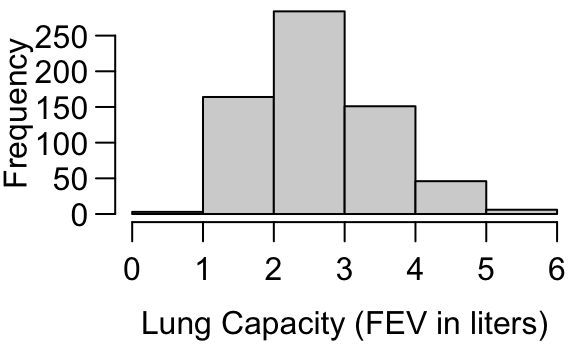
\includegraphics[width=0.5\linewidth]{ch03_24spr_files/figure-beamer/fevhist0-1} \end{center}
\end{frame}

\begin{frame}{Changing Binwidths Can Alter the Shape of a Histogram}
\protect\hypertarget{changing-binwidths-can-alter-the-shape-of-a-histogram}{}
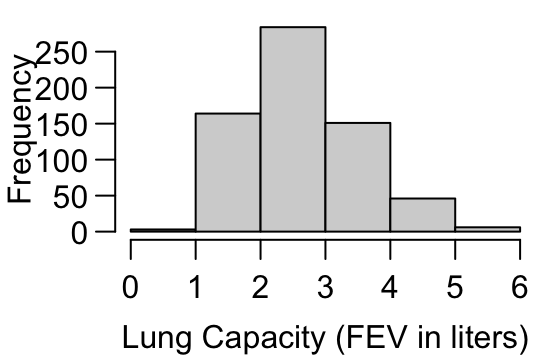
\includegraphics[width=0.48\linewidth]{ch03_24spr_files/figure-beamer/fevhist3-1}
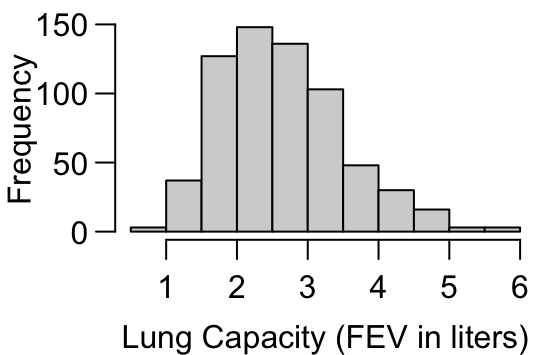
\includegraphics[width=0.48\linewidth]{ch03_24spr_files/figure-beamer/fevhist3-2}
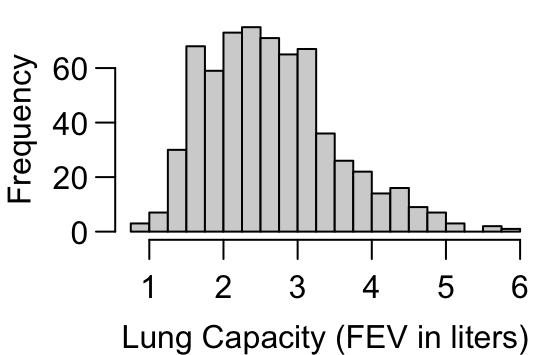
\includegraphics[width=0.48\linewidth]{ch03_24spr_files/figure-beamer/fevhist3-3}
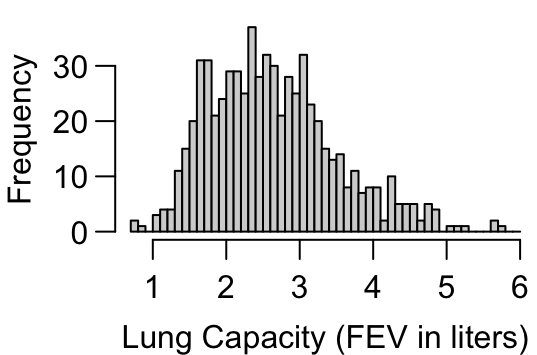
\includegraphics[width=0.48\linewidth]{ch03_24spr_files/figure-beamer/fevhist3-4}
\end{frame}

\begin{frame}{Selection of Binwidth}
\protect\hypertarget{selection-of-binwidth}{}
It is an iterative process --- try and try again.\bigskip

What binwidth should you use?

\begin{itemize}
\tightlist
\item
  Not too small that most bins have either 0 or 1 counts
\item
  Not too big that you lose the details in a bin
\item
  (There may not be a unique ``perfect'' bin size) \vspace{20pt}
\end{itemize}

General rule: \textbf{the more observations, the more bins}.
\end{frame}

\begin{frame}{Skewness of Histograms}
\protect\hypertarget{skewness-of-histograms}{}

\includegraphics[width=1\linewidth]{ch03_24spr_files/figure-beamer/unnamed-chunk-3-1}

\begin{center}
\red{Direction of Skewness = Direction of the Longer Tail}
\end{center}
\end{frame}

\begin{frame}{Mode of Histograms (\(=\) Number of Peaks)}
\protect\hypertarget{mode-of-histograms-number-of-peaks}{}
\begin{center}
\includegraphics[width=0.82\linewidth]{ch03_24spr_files/figure-beamer/unnamed-chunk-4-1} \end{center}

Two or more modes indicate data might come from two or more distinct
populations.
\end{frame}

\begin{frame}{Outliers}
\protect\hypertarget{outliers}{}
We can also check if there are any unusual observations or potential
\hl{outliers} from a histogram.


\includegraphics[width=0.9\linewidth]{ch03_24spr_files/figure-beamer/unnamed-chunk-5-1}

Outliers could be unusual observations or mistakes. Check them!
\end{frame}

\begin{frame}{Comparing Histograms (1)}
\protect\hypertarget{comparing-histograms-1}{}
Here are the histograms of the midterm and the final exam scores for a
class of Elementary Statistics students.\newline  Which exam scores are
generally higher, midterm or final?

\begin{center}
\includegraphics[width=0.9\linewidth]{ch03_24spr_files/figure-beamer/unnamed-chunk-6-1} \end{center}

\pause Key: compare the x-axis!
\end{frame}

\begin{frame}{Comparing Histograms (2)}
\protect\hypertarget{comparing-histograms-2}{}
Which exam scores are generally higher, midterm or final?

\begin{center}
\includegraphics[width=0.9\linewidth]{ch03_24spr_files/figure-beamer/unnamed-chunk-7-1} \end{center}

\pause Key: The average would be higher if bars for higher values have
more observations, and bars for lower values have fewer observations,
\end{frame}

\begin{frame}{Comparing Histograms (3)}
\protect\hypertarget{comparing-histograms-3}{}
Did smokers or nonsmokers have greater lung capacities in general?

\begin{center}
\includegraphics[width=1\linewidth]{ch03_24spr_files/figure-beamer/unnamed-chunk-8-1} \end{center}

\pause\scriptsize

When wo histograms have unequal numbers of observations, we cannot
determine which one has an higher mean by comparing the heights of bars.
This explains the need of histogram in density scale.
\end{frame}

\begin{frame}{Comparing Histograms (4)}
\protect\hypertarget{comparing-histograms-4}{}
Below are the histograms of the birth weights (lbs) of 1000 randomly
sampled babies born in NC in 2024, classified by mother's smoking
status.

Which group had a higher birth weights in general, babies of smoking
moms or those of nonsmoking moms?

\begin{center}
\includegraphics[width=0.9\linewidth]{ch03_24spr_files/figure-beamer/unnamed-chunk-9-1} \end{center}
\end{frame}

\begin{frame}{Back to Smoking \& Birthweight}
\protect\hypertarget{back-to-smoking-birthweight}{}
\begin{minipage}{.45\textwidth}
Did babies born to smoking or nonsmoking mothers
have a higher birthweights?
\end{minipage}

\vspace{-1in}

\begin{flushright}
\includegraphics[width=0.55\linewidth]{ch03_24spr_files/figure-beamer/unnamed-chunk-15-1} \end{flushright}
\end{frame}

\begin{frame}{Histogram in Density Scale}
\protect\hypertarget{histogram-in-density-scale}{}
So far we only introduced histograms in \hl{frequency} scale, of which
the bar height represents the \textbf{count} of \textbf{frequency} of
observations in the class interval (bin).

For histogram in \hl{density} scale,

\begin{center}
\textbf{bar area} $=$ \textbf{percentage} of observations in the bin.
\end{center}

Hence bar height
\(= \dfrac{\text{\% of observations in the bin}}{(\text{bin width})}\)
\end{frame}

\begin{frame}{}
\protect\hypertarget{section}{}
\begin{center}\small
\begin{tabular}{cccc}
Interval & Count & Proportion $=\frac{\text{Count}}{\text{Total}}$ & Bar Height $=\frac{\text{Proportion}}{\text{Bin Width}}$\\\hline
0.5-1 & ~~3 & $\frac{ 3}{654}\approx0.46\%$ & $\frac{0.46}{0.5}=0.92$\\
1-1.5 & ~37 & $\frac{37}{654}\approx5.66\%$ & $\frac{5.66}{0.5}=11.31$\\
1.5-2 & 127 & $\frac{127}{654}\approx19.42\%$ & $\frac{19.42}{0.5}=38.84$\\
2-2.5 & 148 & $\frac{148}{654}\approx22.63\%$ & $\frac{22.63}{0.5}=45.26$\\
$\vdots$ & $\vdots$ & $\vdots$ & $\vdots$\\
5.5-6 & ~~3 & $\frac{3}{654}\approx0.46\%$ & $\frac{0.45}{0.5}=0.92$\\\hline
Total & 654 & 100\% &
\end{tabular}
\end{center}


\includegraphics[width=0.48\linewidth]{ch03_24spr_files/figure-beamer/unnamed-chunk-10-1}
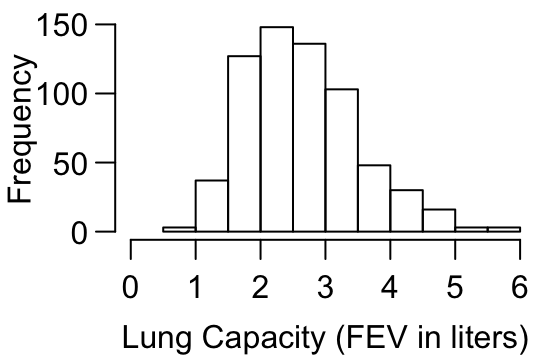
\includegraphics[width=0.48\linewidth]{ch03_24spr_files/figure-beamer/unnamed-chunk-10-2}
\end{frame}

\begin{frame}{Area Under a Histogram = Proportion}
\protect\hypertarget{area-under-a-histogram-proportion}{}
In density scale,

\vspace{-10pt}\begin{center}\tabcolsep=12pt
\begin{tabular}{cc}
Blue \hl{area} = \hl{percentage} of  & Blue \hl{area} = \hl{percentage} of \\
 subjects with FEV  & subjects with FEV \\
 between 0.5 to 2.0             & between 2.0 and 4.0 \\
\end{tabular}
\end{center}


\includegraphics[width=0.48\linewidth]{ch03_24spr_files/figure-beamer/unnamed-chunk-11-1}
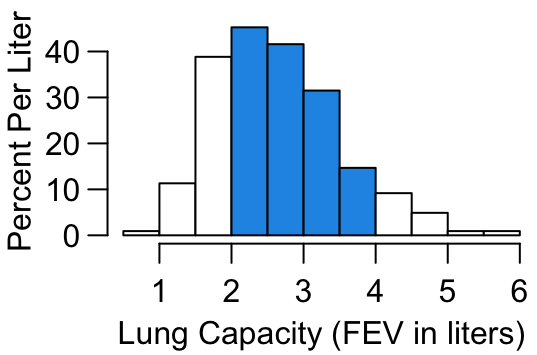
\includegraphics[width=0.48\linewidth]{ch03_24spr_files/figure-beamer/unnamed-chunk-11-2}

In the density scale, the total area under a histogram is 100\% (why?).
\end{frame}

\begin{frame}{Exercise 1 (Number of Cigarettes)}
\protect\hypertarget{exercise-1-number-of-cigarettes}{}
The histogram below shows the number of cigarettes smoked per day for
male current smokers in a public health study.\newline The density (bar
height) is marked in parentheses. \newline The class intervals include
the right endpoint, but not the left.

\begin{center}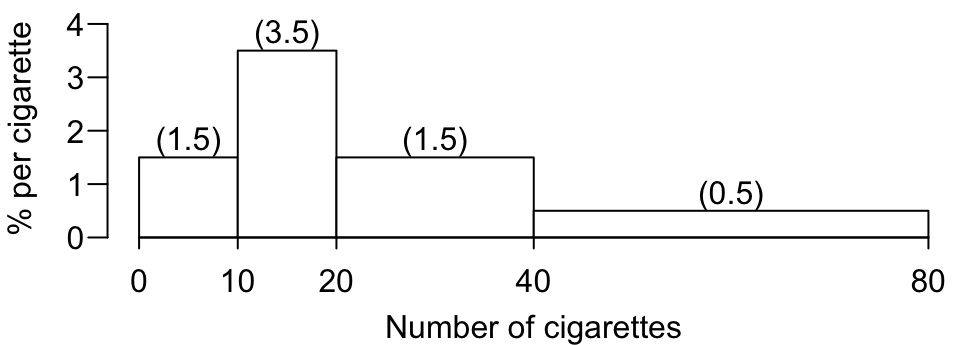
\includegraphics[width=0.85\linewidth]{ch03_24spr_files/figure-beamer/numcigarettes-1} \end{center}

\begin{enumerate}
\tightlist
\item
  The percentage who smoked 10 cigarettes or less per day is around
  \Hide{2-}{$1.5\%\times 10=15\%$}
\end{enumerate}
\end{frame}

\begin{frame}{}
\protect\hypertarget{section-1}{}
\begin{center}
\includegraphics[width=0.85\linewidth]{ch03_24spr_files/figure-beamer/unnamed-chunk-12-1} \end{center}

\begin{enumerate}
\setcounter{enumi}{1}
\item
  The percentage who smoked more than a pack a day, but not more than 2
  packs, is around \Hide{2-}{$1.5\%\times 20=30\%$}\newline (A pack
  \(=\) 20 cigarettes)
\item
  The percent who smoked more than a pack a day is around
  \Hide{3-}{$1.5\%\times 20+0.5\%\times40=50\%$}
\item
  The percent who smoked more than 3 packs a day is around
  \Hide{4-}{$0.5\%\times 20=10\%$}
\end{enumerate}
\end{frame}

\begin{frame}{Exercise 2 (Wages)}
\protect\hypertarget{exercise-2-wages}{}
Below is a histogram of weekly wages for part-time employees. Nobody
earned more than \$1,000 a week. The block over the class interval
\$200-\$500 is missing. How tall must it be?

\begin{center}
\includegraphics[width=0.8\linewidth]{ch03_24spr_files/figure-beamer/unnamed-chunk-13-1} \end{center}
\vspace{-8pt}

\begin{itemize}
\tightlist
\item
  1 unit in the horizontal scale \(=\) \Hide{2-}{\$100}.
\item
  Remember: the total area of a histogram is \Hide{3-}{100\%}.
\item
  Area of the missing block = \Hide{4-}{45\%}.
\item
  Height of the missing block = \Hide{5-}{$45\%/3=15\%$}.
\end{itemize}
\end{frame}

\begin{frame}{Back to FEV Data}
\protect\hypertarget{back-to-fev-data}{}
\begin{minipage}{.45\textwidth}
Stacking histograms vertically makes it easier
to \textbf{compare the horizontal scale}.\vspace{0.6in}

Did smokers or nonsmokers have greater lung capacities in general?

\end{minipage}

\vspace{-2in}

\begin{flushright}
\includegraphics[width=0.55\linewidth]{ch03_24spr_files/figure-beamer/unnamed-chunk-14-1} \end{flushright}
\end{frame}

\begin{frame}{Back to Smoking \& Birthweight}
\protect\hypertarget{back-to-smoking-birthweight}{}
\begin{minipage}{.45\textwidth}
Did babies born to smoking or nonsmoking mothers
have a higher birthweights?
\end{minipage}

\vspace{-1in}

\begin{flushright}
\includegraphics[width=0.55\linewidth]{ch03_24spr_files/figure-beamer/unnamed-chunk-15-1} \end{flushright}
\end{frame}

\begin{frame}{Summary of Histograms}
\protect\hypertarget{summary-of-histograms}{}
What to Look in a Histogram?

\begin{itemize}
\item
  \textbf{Shape}

  \begin{itemize}
  \tightlist
  \item
    symmetric or skewed (lopsided)
  \item
    number of modes (peaks)
  \end{itemize}
\item
  \textbf{Outliers}
\item
  \textbf{Center}: Where is the ``middle'' of the histogram?

  \begin{itemize}
  \tightlist
  \item
    typically represented by \emph{average} and \emph{median}
  \end{itemize}
\item
  \textbf{Spread}: What big the range the data spread?

  \begin{itemize}
  \tightlist
  \item
    typically represented by \emph{SD} and \emph{IQR} (will introduce
    soon)
  \end{itemize}
\end{itemize}

Keep in mind that

\begin{center}
 \fbox{Area Under a Histogram $=$ Percentage}
\end{center}
\end{frame}

\end{document}
